\chapter{Аугментация предобученных моделей}\label{ch:ch3}

\section{Кодировщик}\label{sec:ch3/sect1}

Для проверки нашего подхода в условиях реального применения мы используем популярный бенчмарк Hyperpartisan news для классификации длинных текстов \cite{kiesel2019semeval}. Вместо обучения модели RMT с нуля мы добавляем механизм рекуррентной памяти к наиболее распространенным моделям из библиотеки HuggingFace Transformers \cite{wolf2020transformers}. В частности, предварительно обученные модели BERT-base, RoBERTa-base, DeBERTa-base и T5-base были дополнены памятью размером 10, увеличивающей входные данные из 500 токенов, и дообучены на целевой задаче.

\begin{table}
\centering
\begin{tabular}{lcccc}
\hline
\multirow{2}{*}{Model (input size)} & \multicolumn{4}{c}{Number of segments} \\
                                    & 1         & 2         & 3         & 4         \\
\hline
Big Bird (4096) \cite{zaheer2020big} & 92.20     &           &           &           \\
Longformer (4096) \cite{beltagy2020longformer} & 94.80     &           &           &           \\
Graph-roberta (512x100) \cite{xu2021contrastive} & 96.15     &           &           &           \\
ERNIE-DOC-Large (640) \cite{ding-etal-2021-ernie-doc} & \underline{96.60} &           &           &           \\
ERNIE-Sparse (4096) \cite{liu2022ernie} & 92.81     &           &           &           \\
\hline
RMT bert-base-case (512) & 91.60 & 94.12 & 93.06 & 94.34 \\
RMT roberta-base (512) & 94.87 & \textbf{97.20} & \textbf{96.72} & \underline{\textbf{98.11}} \\
RMT deberta-v3-base (512) & 94.17 & 96.78 & 94.80 & 94.80 \\
RMT t5-base (512) & \textbf{94.99} & 95.32 & 96.12 & 97.20 \\
\hline
\end{tabular}
\caption{\textbf{Hyperpartisan news detection.} Models starting with RMT are taken from HuggingFace Transformers and augmented with 10 memory tokens and recurrence before fine-tuning. Train/valid/test split as in \cite{beltagy2020longformer} and metric is F1.}
\label{tab:hyp}
\end{table}    


Предложенный механизм рекуррентной памяти изменяет только обработку входа и градиентные потоки в дополненных моделях. Это дает существенное преимущество, так как память можно легко интегрировать в уже обученные модели. Как показано в \cref{tab:hyp}, результаты оценки демонстрируют производительность четырех моделей с дополненной памятью, дообученных для классификации длинных текстов. Включение 10 токенов памяти во входную последовательность длиной 512 токенов позволяет обрабатывать тексты длиной до 2000 токенов и существенно повышает метрики у большинства моделей. Особенно примечательно, что сочетание рекуррентной памяти с RoBERTa-base обеспечивает лучшие результаты для задачи классификации Hyperpartisan news \cite{kiesel2019semeval}. При этом конкурирующие модели с длиной входной последовательности 4096 токенов — что более чем в два раза превышает расширенный вход RMT — демонстрируют более низкую производительность.


\section{Memorization Tasks}


Для изучения способности запоминать, мы создали наборы синтетических данных, которые требуют воспроизведения простых фактов и выполнения базовых логических операций. В каждой задаче подаются один или несколько фактов вместе с вопросом, ответ на который возможен только при использовании всех предоставленных фактов. Чтобы усложнить задачи, в текст добавляются дополнительные фрагменты естественного языка, не связанные с вопросами или ответами. Модель должна различить факты среди отвлекающего текста, чтобы дать правильный ответ. Эти задачи оформлены как классификация с шестью классами, где каждый класс соответствует определенному ответу.

Факты взяты из набора данных bAbI \cite{WestonBCM15}, а отвлекающий текст заимствован из длинных вопросов из датасета QuALITY \cite{pang-etal-2022-quality}.

\begin{verbatim}
Background text: ... He was a big man, broad-shouldered and still thin-waisted. 
Eddie found it easy to believe the stories he had heard about his father ...
\end{verbatim}

\begin{figure}
\centering
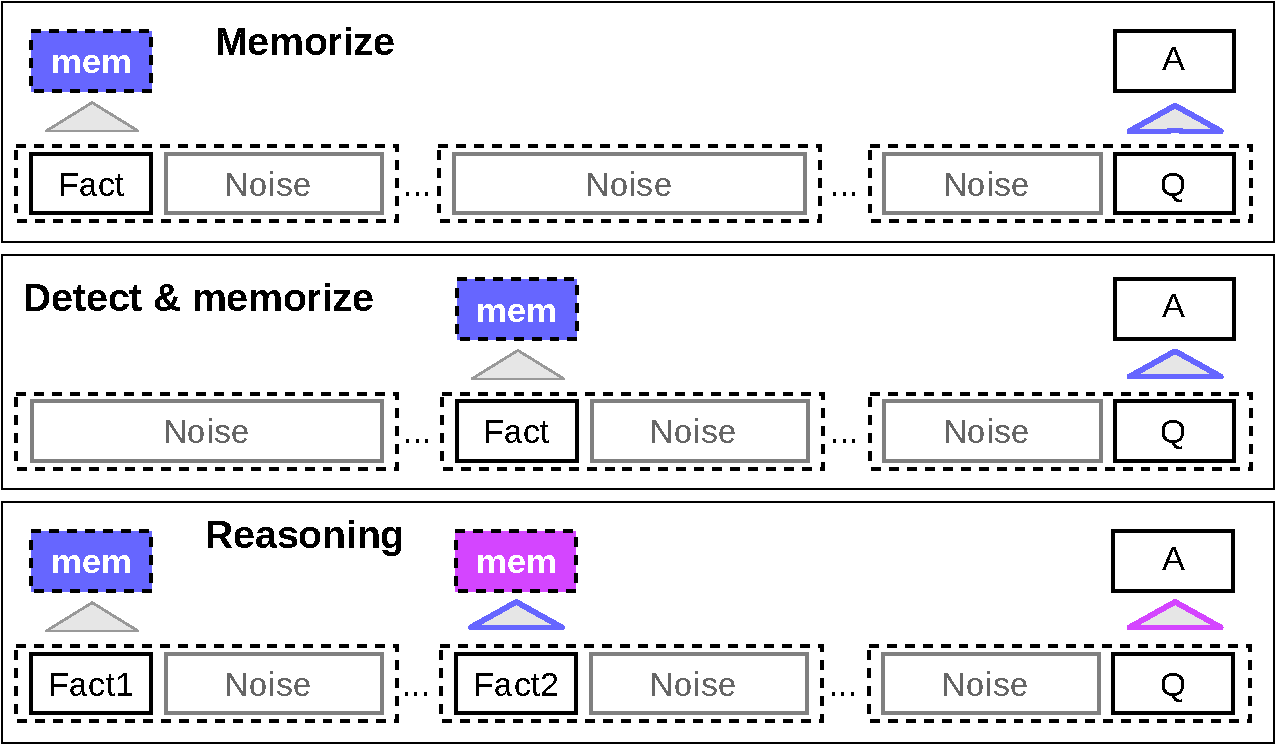
\includegraphics[width=0.65\linewidth]{images/part3/rmt_tasks_simple.pdf}
\caption{\small\textbf{Синтетические задачи, требующие памяти.} На графике представлены задачи и необходимые для их выполнения операции памяти в рамках RMT. В задаче "Запоминание" факты размещены в начале текста. Задача "Обнаружение и запоминание" усложняется случайным расположением фактов в тексте. В задаче "Логика" используется два случайных факта для ответа на финальный вопрос. Вопрос в каждой задаче всегда находится в конце текста.}
\label{tasks-approaches}
\end{figure}


Первая задача проверяет способность RMT сохранять информацию в памяти на протяжении длительного времени (Рисунок~\ref{tasks-approaches}, верх). На начальном уровне факт всегда размещается в начале последовательности, а вопрос — в конце. Количество нерелевантного текста между фактами и вопросом постепенно увеличивается до тех пор, пока длина текста не превысит объем ввода модели.

\begin{verbatim}
Fact: Daniel went back to the hallway.
Question: Where is Daniel?
Answer: hallway
\end{verbatim}

"Обнаружение и запоминание" представляет собой более сложную задачу, где факт случайным образом помещается в текст (Рисунок~\ref{tasks-approaches}, середина). Модели необходимо сначала выделить нужный факт из отвлекающего текста, записать его в память, а затем использовать для ответа на вопрос.

Для проверки работы с несколькими фактами мы разработали сложную задачу "Логика". Здесь требуется два факта, которые случайно распределяются в тексте, а вопрос построен так, чтобы требовать взаимосвязи между ними. Эта задача аналогична \textit{Two Argument Relation} из bAbI (Рисунок~\ref{tasks-approaches}, низ).

\begin{verbatim}
Fact1: The hallway is east of the bathroom.
Fact2: The bedroom is west of the bathroom.
Question: What is the bathroom east of?
Answer: bedroom
\end{verbatim}

\section{Learning Memory Operations}

В рамках экспериментов мы использовали предварительно обученные модели из библиотеки Hugging Face Transformers \cite{wolf2020transformers}. Они были дополнены модулями памяти и обучены с применением оптимизатора AdamW \cite{loshchilov2018adamw} с линейным изменением скорости обучения и фазой разогрева. Подробности о гиперпараметрах и скрипты для воспроизведения экспериментов будут доступны в приложении и на GitHub.

Эксперименты проводились на 4-8 видеокартах Nvidia 1080ti. Для оценки длинных последовательностей использовалась одна Nvidia A100 с 40 ГБ памяти.

\begin{figure}
\centering
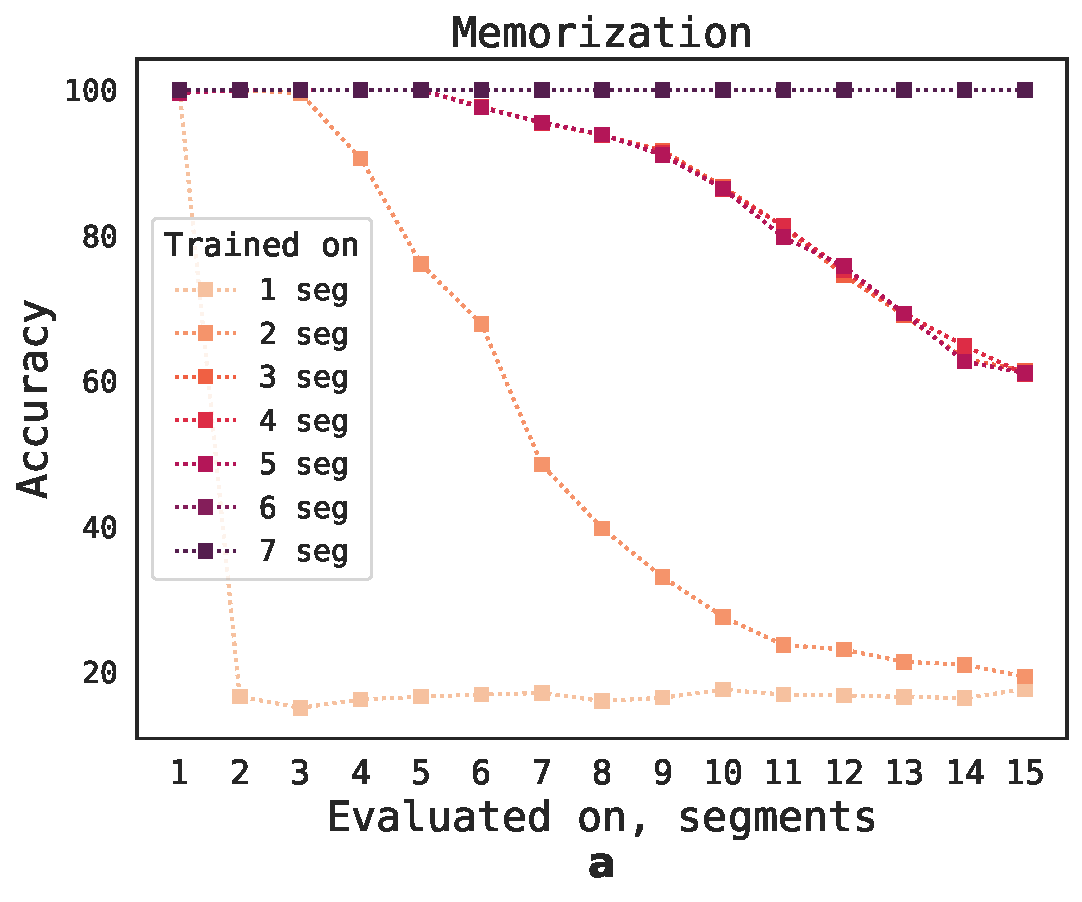
\includegraphics[width=0.45\linewidth]{images/part3/extrapolate.pdf}
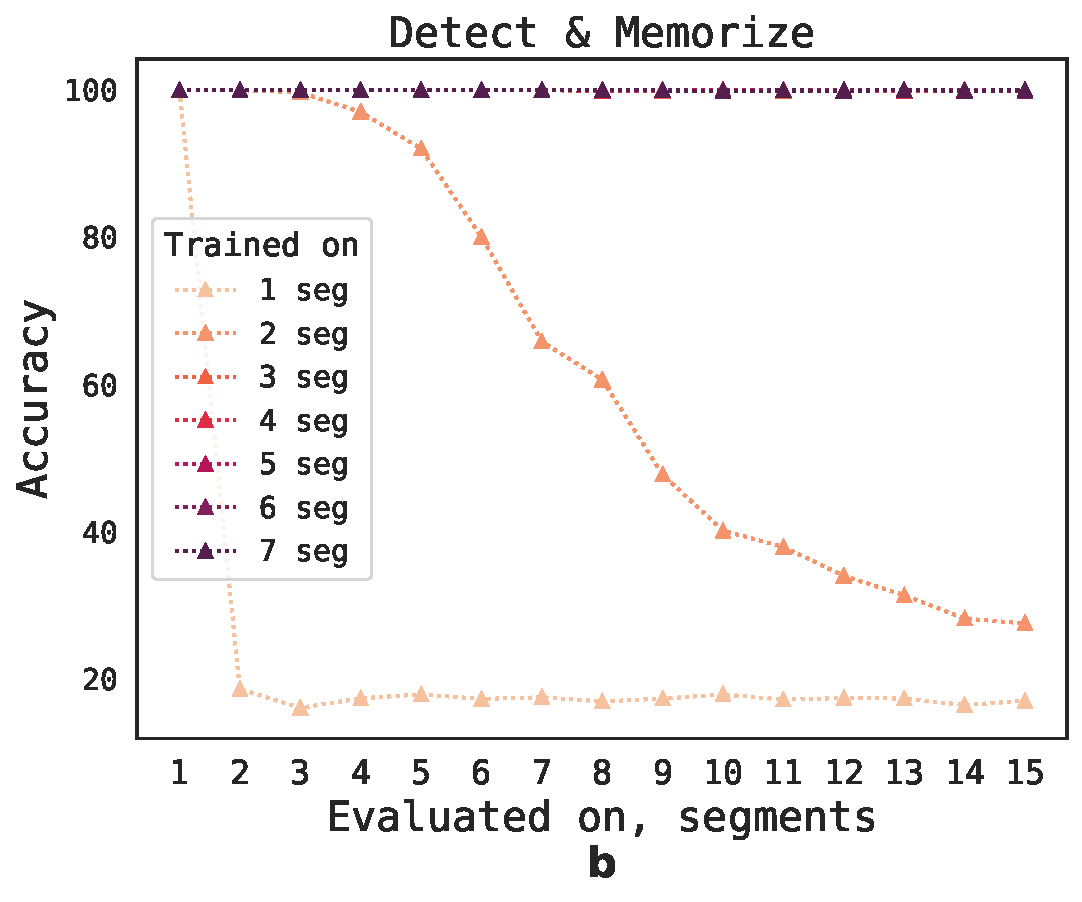
\includegraphics[width=0.45\linewidth]{images/part3/extrapolate_random.pdf} \
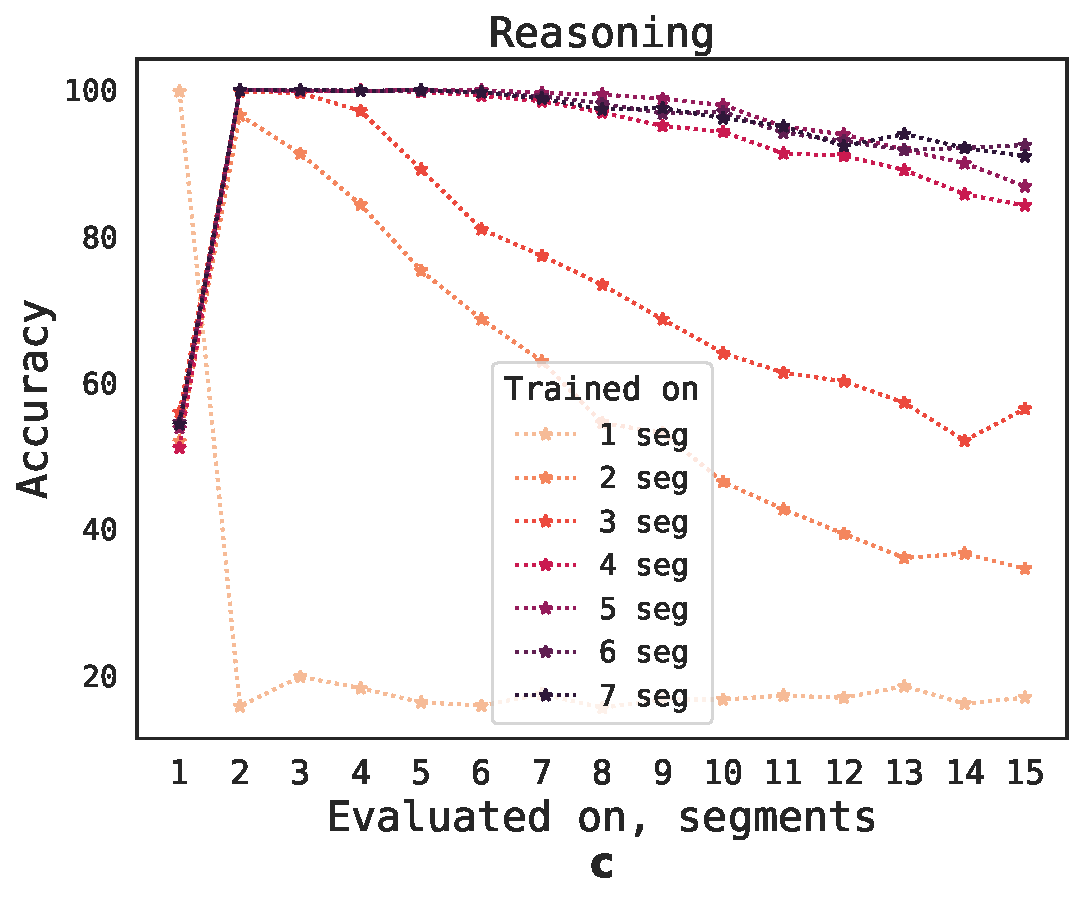
\includegraphics[width=0.45\linewidth]{images/part3/extrapolate_reason.pdf}
\caption{\small\textbf{Обобщение операций извлечения из памяти.} Обученные модели оценивались на задачах с длиной последовательностей от 1 до 7 сегментов с размером памяти 10. \textbf{a}: Запоминание, \textbf{b}: Обнаружение, \textbf{c}: Логика. Модели, натренированные на 5+ сегментах, демонстрируют отличную способность к обобщению для более длинных входных данных.}
\label{extrapolate}
\end{figure}


\subsection{Curriculum Learning}

Мы обнаружили, что использование последовательного подхода к обучению значительно повышает стабильность работы модели и точность её решений. На начальном этапе RMT обучается на укороченных версиях задачи. После того как модель достигает сходимости, задача постепенно усложняется за счёт добавления нового сегмента. Такой подход продолжается до тех пор, пока не будет достигнута целевая длина входной последовательности.

В наших экспериментах обучение начинается с последовательностей, умещающихся в один сегмент. Реальный размер сегмента составляет 499 токенов, так как от доступных 512 токенов выделяются 3 для специальных символов BERT и 10 для управления памятью. Обучение на укороченных задачах помогает RMT эффективнее справляться с более длинными версиями, сокращая количество шагов, необходимых для достижения оптимального результата.

\begin{figure}[t]
\centering
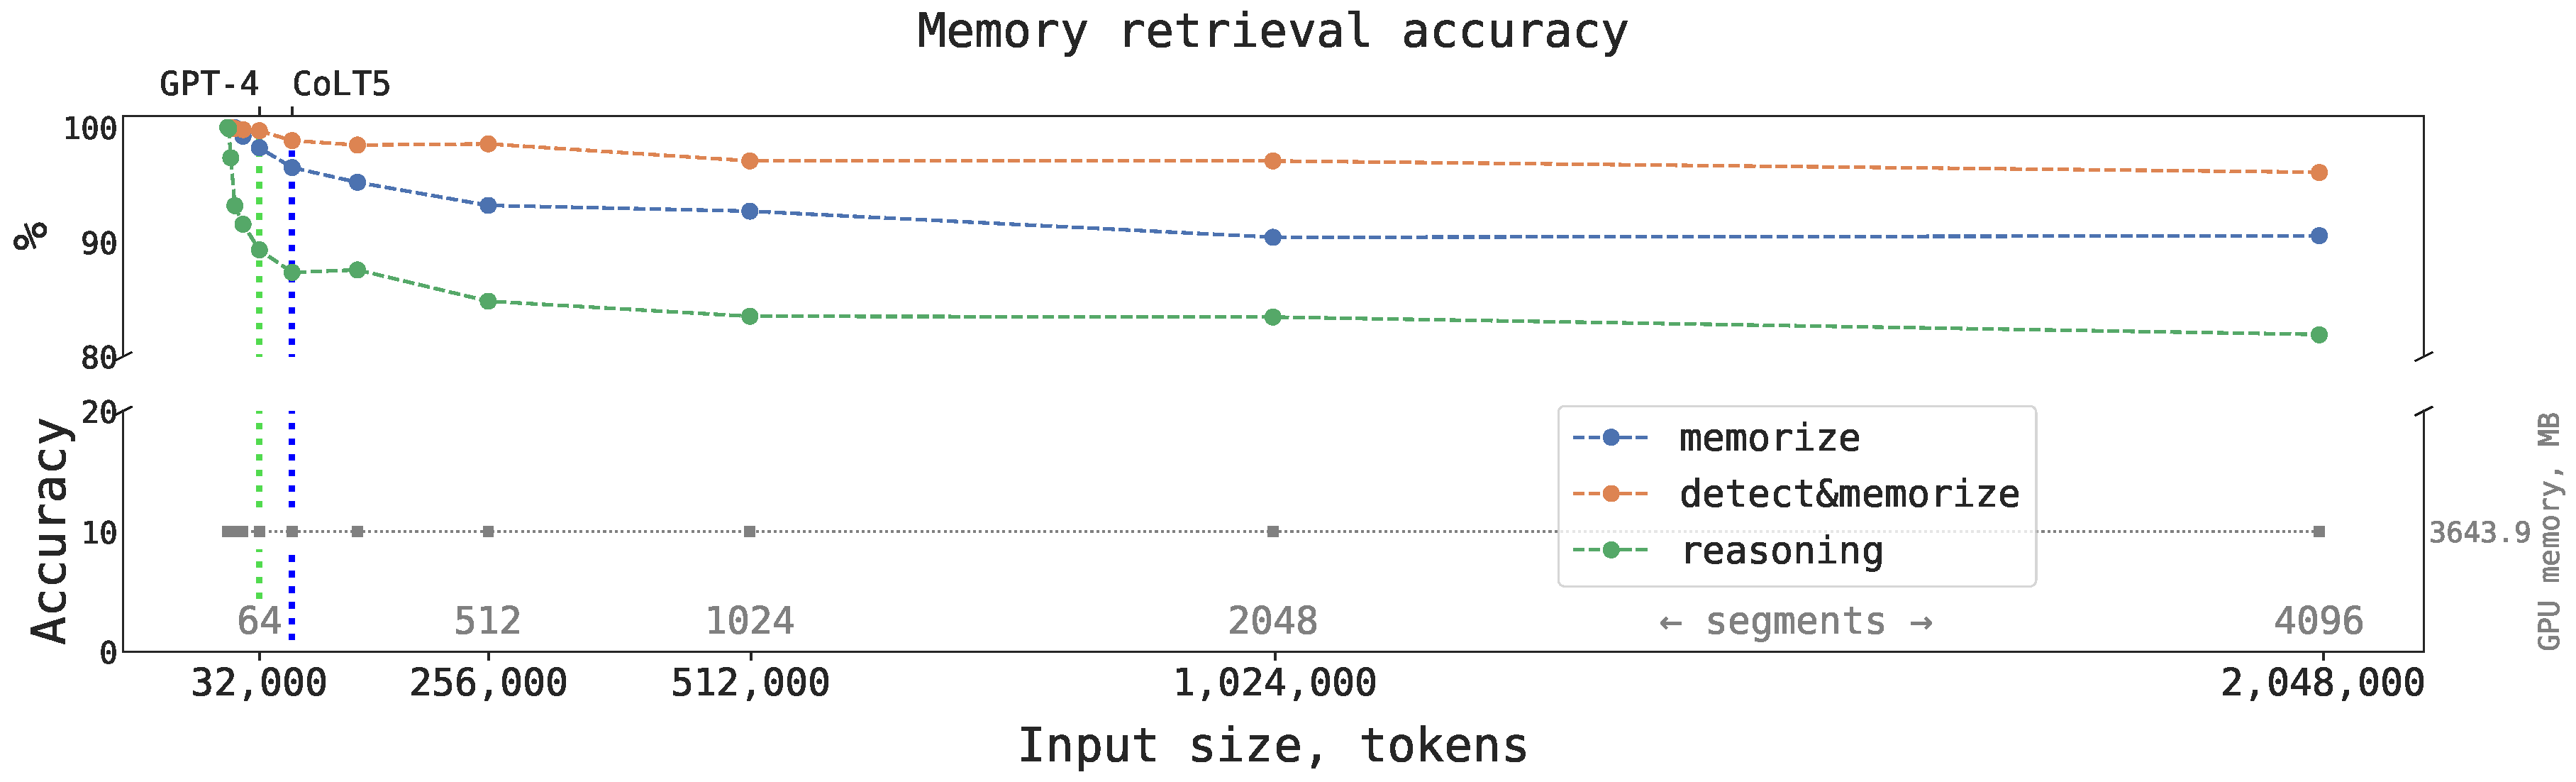
\includegraphics[width=\linewidth]{images/part3/extrapolate_long_log+tok_linear.pdf}
\caption{\small\textbf{Рекуррентный Memory Transformer способен хранить информацию на последовательностях длиной до $2\times10^6$ токенов}. Интеграция механизма рекуррентной памяти в предварительно обученную модель BERT \cite{bulatov2022recurrent} позволяет сохранять информацию о задаче в семи сегментах по 512 токенов каждый. На этапе инференса модель эффективно обрабатывает 4,096 сегментов, что соответствует общей длине последовательности в 2,048,000 токенов. Это значительно превосходит максимальные размеры входных данных ранее известных трансформеров, таких как 64K токенов для CoLT5 \cite{ainslie2023colt5}, 32K для GPT-4 \cite{openai2023gpt4} и 100K для Claude. Важно отметить, что расширение выполняется без увеличения размера памяти базовой модели, который в экспериментах составляет 3,6 ГБ.}
\label{extrapolate-long}
\end{figure}

\subsection{Extrapolation Abilities}
\label{sec:extrapolation_abilites}

Как хорошо RMT справляется с последовательностями различной длины? Чтобы изучить этот вопрос, мы тестировали модели, обученные на разном количестве сегментов, для выполнения задач с увеличенной длиной (рис.~\ref{extrapolate}). Результаты показывают, что модели успешно справляются с короткими задачами, за исключением случая односегментной задачи рассуждения. При увеличении длины обучения модель перестаёт ожидать появления вопроса в первом сегменте, что снижает точность.

Однако способность модели к обобщению улучшается с увеличением числа сегментов в обучении. Так, модели, обученные на пяти или более сегментах, демонстрируют почти идеальную генерализацию на задачах вдвое длиннее обучающих. Чтобы определить пределы этой способности, мы протестировали задачи длиной до 4,096 сегментов (2,043,904 токена). Даже на таких длинных последовательностях RMT показывает хорошие результаты: задачи на "обнаружение и запоминание" выполняются легче всего, в то время как задачи рассуждения требуют больше ресурсов.

\begin{figure}[h]
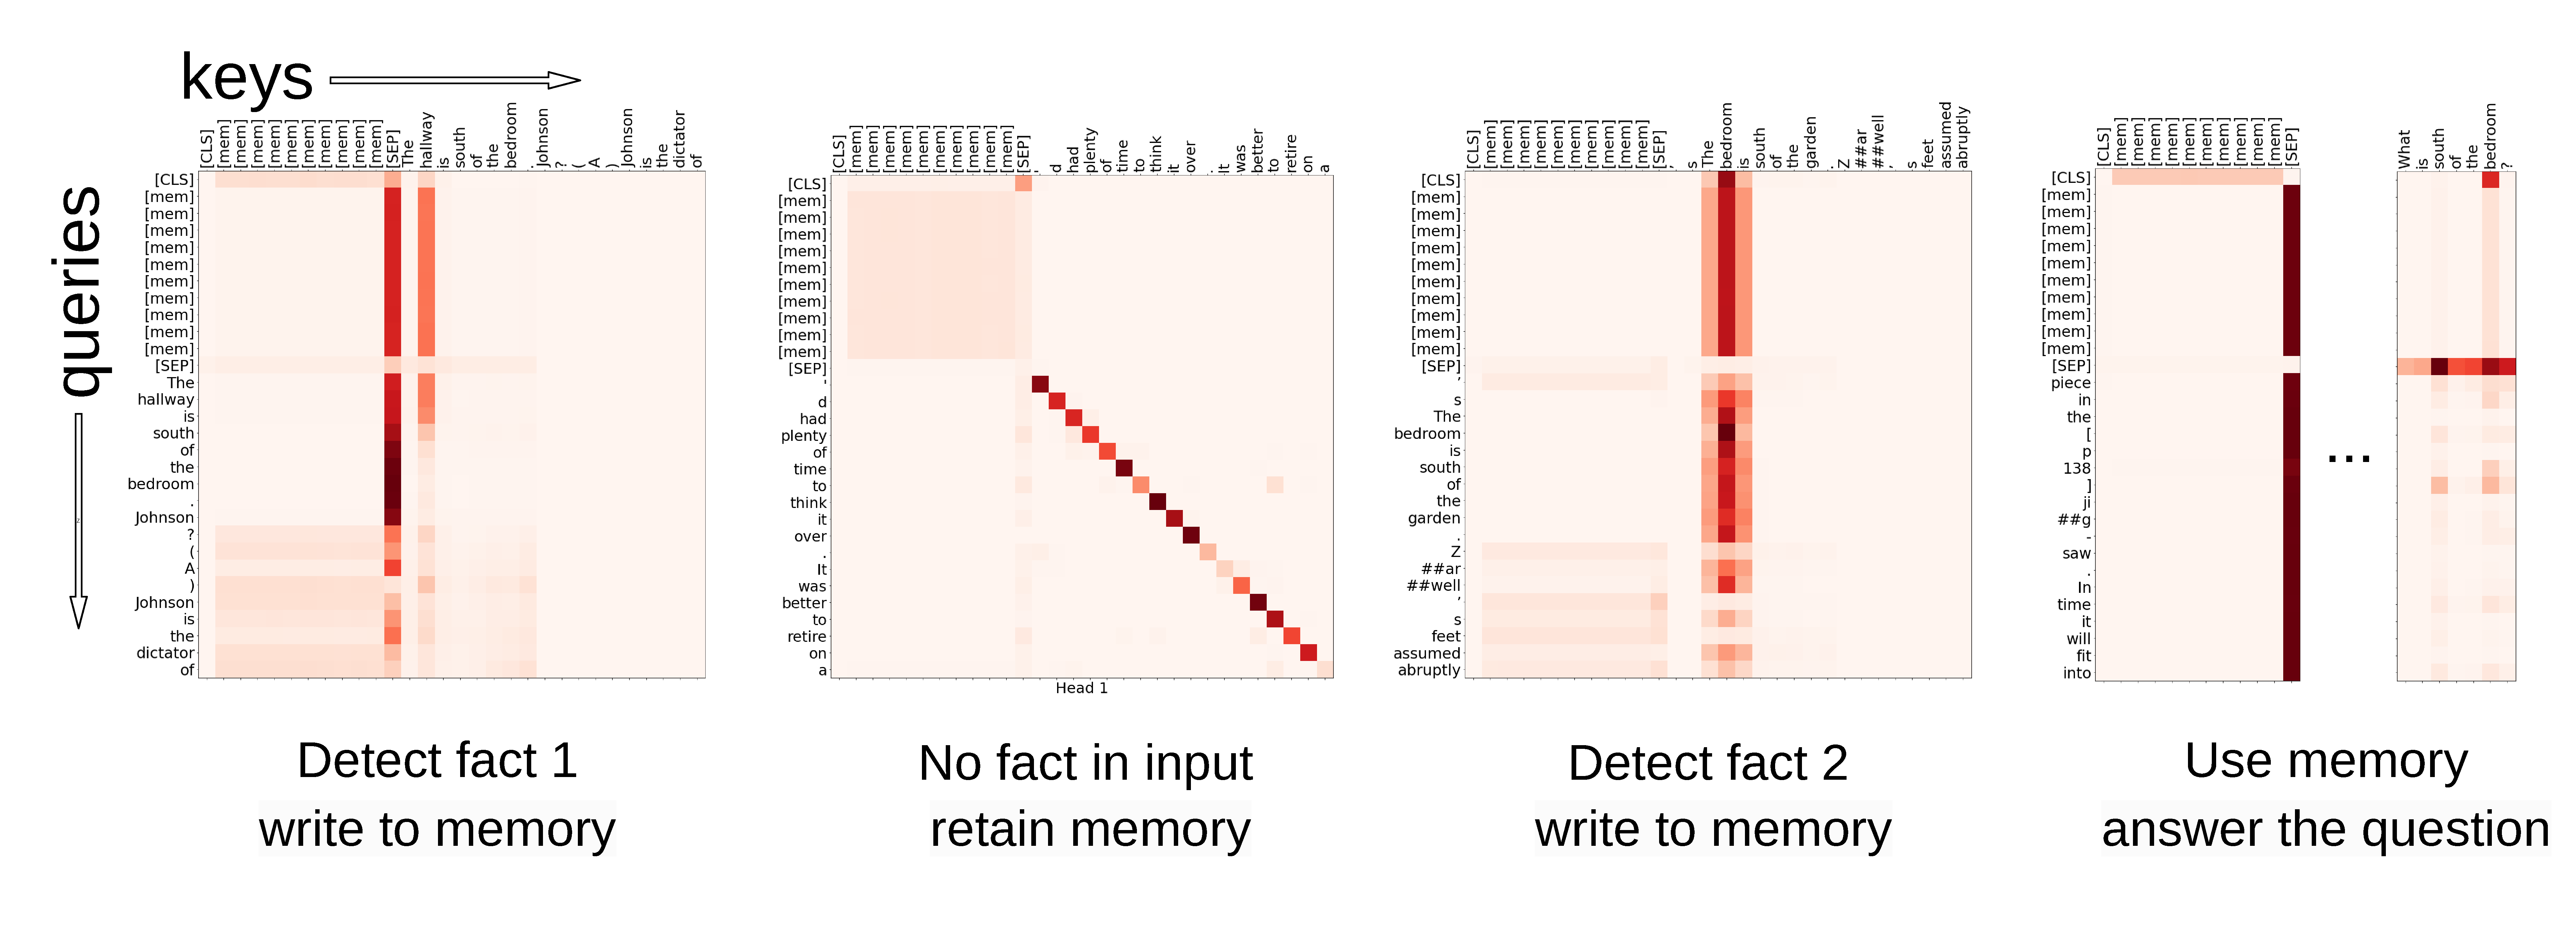
\includegraphics[width=1\linewidth]{images/part3/rmt-basic-attention-maps-v3.pdf}
\caption{\small\textbf{Карты внимания для работы с памятью}. На тепловых картах показаны механизмы внимания в процессе выполнения четырёхсегментной задачи рассуждения. Интенсивность пикселей соответствует значению внимания между ключами и значениями. Слева направо: модель обнаруживает первый факт и записывает его в память ([mem]-токены); второй сегмент не содержит полезной информации, поэтому содержимое памяти остаётся неизменным; модель находит второй факт и добавляет его в память; CLS извлекает из памяти информацию для ответа на вопрос.}
\label{mem_operations}
\end{figure}

Анализ тепловых карт внимания RMT (рис.~\ref{mem_operations}) показывает, что операции с памятью связаны с конкретными паттернами внимания. Высокие результаты экстраполяции на экстремально длинных последовательностях, обсуждаемые в разделе~\ref{sec:extrapolation_abilites}, подтверждают эффективность выученных операций с памятью, даже при их многократном использовании. Примечательно, что RMT управляет памятью без специальных модулей чтения или записи: трансформер самостоятельно обучается рекуррентному взаимодействию с памятью. Этот результат особенно впечатляет, учитывая, что такие операции с памятью не были напрямую мотивированы функцией потерь задачи. 


\section{Декодировщики}\label{sec:ch3/sect2}


% \begin{table*}[t!]
% \footnotesize
% \scalebox{0.87}{
%     \begin{tabular}
%     \end{tabular}
% }

% \vspace{1mm}
% \caption{}
% \label{}
% \end{table*}

